\documentclass[10pt,twocolumn]{article}
% Shared two-column preamble for the three research papers.
% Use with: \documentclass[10pt,twocolumn]{article}
% Then in main.tex: % Shared two-column preamble for the three research papers.
% Use with: \documentclass[10pt,twocolumn]{article}
% Then in main.tex: % Shared two-column preamble for the three research papers.
% Use with: \documentclass[10pt,twocolumn]{article}
% Then in main.tex: \input{../../shared/latex/twocolumn_preamble.tex}

\usepackage[margin=0.75in]{geometry}
\usepackage[utf8]{inputenc}
\usepackage[T1]{fontenc}
\usepackage{lmodern}
\usepackage{microtype}
\usepackage{amsmath,amssymb,amsthm}
\usepackage{graphicx}
\usepackage{booktabs}
\usepackage{caption}
\usepackage{subcaption}
\usepackage{hyperref}
\usepackage{url}
\usepackage{xcolor}
\usepackage{algorithm}
\usepackage{algorithmic}
\usepackage{multirow}
\usepackage{titlesec}
\usepackage{authblk}

\hypersetup{colorlinks=true,linkcolor=blue!50!black,citecolor=blue!50!black,urlcolor=blue!50!black}

\titleformat{\section}{\normalfont\large\bfseries}{\thesection}{0.6em}{}
\titleformat{\subsection}{\normalfont\bfseries}{\thesubsection}{0.5em}{}

\captionsetup{font=small,labelfont=bf,skip=4pt}
\setlength{\columnsep}{0.25in}
\setlength{\parskip}{2pt}

\newtheorem{theorem}{Theorem}
\newtheorem{proposition}[theorem]{Proposition}
\newtheorem{definition}[theorem]{Definition}


\usepackage[margin=0.75in]{geometry}
\usepackage[utf8]{inputenc}
\usepackage[T1]{fontenc}
\usepackage{lmodern}
\usepackage{microtype}
\usepackage{amsmath,amssymb,amsthm}
\usepackage{graphicx}
\usepackage{booktabs}
\usepackage{caption}
\usepackage{subcaption}
\usepackage{hyperref}
\usepackage{url}
\usepackage{xcolor}
\usepackage{algorithm}
\usepackage{algorithmic}
\usepackage{multirow}
\usepackage{titlesec}
\usepackage{authblk}

\hypersetup{colorlinks=true,linkcolor=blue!50!black,citecolor=blue!50!black,urlcolor=blue!50!black}

\titleformat{\section}{\normalfont\large\bfseries}{\thesection}{0.6em}{}
\titleformat{\subsection}{\normalfont\bfseries}{\thesubsection}{0.5em}{}

\captionsetup{font=small,labelfont=bf,skip=4pt}
\setlength{\columnsep}{0.25in}
\setlength{\parskip}{2pt}

\newtheorem{theorem}{Theorem}
\newtheorem{proposition}[theorem]{Proposition}
\newtheorem{definition}[theorem]{Definition}


\usepackage[margin=0.75in]{geometry}
\usepackage[utf8]{inputenc}
\usepackage[T1]{fontenc}
\usepackage{lmodern}
\usepackage{microtype}
\usepackage{amsmath,amssymb,amsthm}
\usepackage{graphicx}
\usepackage{booktabs}
\usepackage{caption}
\usepackage{subcaption}
\usepackage{hyperref}
\usepackage{url}
\usepackage{xcolor}
\usepackage{algorithm}
\usepackage{algorithmic}
\usepackage{multirow}
\usepackage{titlesec}
\usepackage{authblk}

\hypersetup{colorlinks=true,linkcolor=blue!50!black,citecolor=blue!50!black,urlcolor=blue!50!black}

\titleformat{\section}{\normalfont\large\bfseries}{\thesection}{0.6em}{}
\titleformat{\subsection}{\normalfont\bfseries}{\thesubsection}{0.5em}{}

\captionsetup{font=small,labelfont=bf,skip=4pt}
\setlength{\columnsep}{0.25in}
\setlength{\parskip}{2pt}

\newtheorem{theorem}{Theorem}
\newtheorem{proposition}[theorem]{Proposition}
\newtheorem{definition}[theorem]{Definition}

% auto-generated by src/figures/plot_denoise.py
\newcommand{\DiffGscVsRtf}{+4.5}
\newcommand{\DiffMuteVsRef}{-0.8}
\newcommand{\DiffRefDfnInf}{+16.1}
\newcommand{\DiffRefDfnTwelve}{+2.7}
\newcommand{\DiffRefHomeTwo}{+6.3}
\newcommand{\DiffRtfDfnInf}{+18.5}
\newcommand{\DiffRtfDfnTwelve}{+0.8}
\newcommand{\DiffRtfDfnVsRefDfn}{-26.3}
\newcommand{\DiffRtfHomeTwo}{+11.4}
\newcommand{\DiffRtfVsRef}{-24.4}
\newcommand{\DoaErrSnrFive}{11}
\newcommand{\DoaErrSnrMFive}{65}
\newcommand{\DoaErrSnrOneZero}{5}
\newcommand{\DoaErrSnrZero}{58}
\newcommand{\Gainds}{0.4}
\newcommand{\Gaingsc}{3.7}
\newcommand{\Gainmean}{0.4}
\newcommand{\Gainmute}{0.4}
\newcommand{\Gainmutesoft}{0.5}
\newcommand{\Gainmvdrdoa}{2.9}
\newcommand{\Gainmvdrrtf}{4.3}
\newcommand{\Gainoracle}{9.1}
\newcommand{\Gainref}{0.0}
\newcommand{\LiveGaingsc}{2.4}
\newcommand{\LiveGainmean}{-0.6}
\newcommand{\LiveGainmute}{-0.5}
\newcommand{\LiveGainmvdrdoa}{3.3}
\newcommand{\LiveGainmvdrrtf}{2.9}
\newcommand{\LiveGainref}{0.0}
\newcommand{\LivecafeteriachZerochipDfn}{48}
\newcommand{\LivecafeteriachZerochipOff}{39}
\newcommand{\LivecafeteriagscDfn}{16}
\newcommand{\LivecafeteriagscOff}{16}
\newcommand{\LivecafeteriamuteDfn}{48}
\newcommand{\LivecafeteriamuteOff}{42}
\newcommand{\LivecafeteriamvdrdoaDfn}{16}
\newcommand{\LivecafeteriamvdrdoaOff}{16}
\newcommand{\LivecafeteriamvdrrtfDfn}{16}
\newcommand{\LivecafeteriamvdrrtfOff}{16}
\newcommand{\LivecafeteriarefDfn}{48}
\newcommand{\LivecafeteriarefOff}{35}
\newcommand{\LivetalkerchZerochipDfn}{200}
\newcommand{\LivetalkerchZerochipOff}{200}
\newcommand{\LivetalkergscDfn}{15}
\newcommand{\LivetalkergscOff}{11}
\newcommand{\LivetalkermuteDfn}{207}
\newcommand{\LivetalkermuteOff}{167}
\newcommand{\LivetalkermvdrdoaDfn}{7}
\newcommand{\LivetalkermvdrdoaOff}{11}
\newcommand{\LivetalkermvdrrtfDfn}{11}
\newcommand{\LivetalkermvdrrtfOff}{11}
\newcommand{\LivetalkerrefDfn}{44}
\newcommand{\LivetalkerrefOff}{148}
\newcommand{\NDfnScenes}{80}
\newcommand{\NScenes}{320}
\newcommand{\NTranscripts}{4,016}
\newcommand{\NUtts}{8}
\newcommand{\PFifteenLooErr}{16}
\newcommand{\PFifteenMaeBest}{0.40}
\newcommand{\PFifteenMaeMean}{0.41}
\newcommand{\PFifteenOffset}{35}
\newcommand{\PFifteenSpearmanMax}{0.30}
\newcommand{\PGscVsRtf}{0.04}
\newcommand{\PMuteVsRef}{0.47}
\newcommand{\PRefDfnInf}{$9{\times}10^{-9}$}
\newcommand{\PRefDfnTwelve}{0.46}
\newcommand{\PRefHomeTwo}{$3{\times}10^{-5}$}
\newcommand{\PRtfDfnInf}{$5{\times}10^{-12}$}
\newcommand{\PRtfDfnTwelve}{0.48}
\newcommand{\PRtfDfnVsRefDfn}{$1{\times}10^{-8}$}
\newcommand{\PRtfHomeTwo}{$1{\times}10^{-9}$}
\newcommand{\PRtfVsRef}{$5{\times}10^{-9}$}
\newcommand{\SuperResidual}{-6.4}
\newcommand{\WerAkane}{15}
\newcommand{\WerClean}{15}
\newcommand{\WergscattOneEight}{56}
\newcommand{\WergscattOneTwo}{54}
\newcommand{\WergscattSix}{51}
\newcommand{\WergscattTwoFour}{62}
\newcommand{\Wergscattinf}{72}
\newcommand{\Wergscattoff}{54}
\newcommand{\WermuteattOneEight}{81}
\newcommand{\WermuteattOneTwo}{80}
\newcommand{\WermuteattSix}{74}
\newcommand{\WermuteattTwoFour}{84}
\newcommand{\Wermuteattinf}{91}
\newcommand{\Wermuteattoff}{73}
\newcommand{\WermvdrdoaattOneEight}{61}
\newcommand{\WermvdrdoaattOneTwo}{59}
\newcommand{\WermvdrdoaattSix}{53}
\newcommand{\WermvdrdoaattTwoFour}{65}
\newcommand{\Wermvdrdoaattinf}{74}
\newcommand{\Wermvdrdoaattoff}{54}
\newcommand{\WermvdrrtfHomeTwo}{62}
\newcommand{\WermvdrrtfattOneEight}{52}
\newcommand{\WermvdrrtfattOneTwo}{50}
\newcommand{\WermvdrrtfattOneTwocafeteria}{49}
\newcommand{\WermvdrrtfattOneTwofan}{59}
\newcommand{\WermvdrrtfattOneTwomusic}{24}
\newcommand{\WermvdrrtfattOneTwopink}{59}
\newcommand{\WermvdrrtfattOneTwotalker}{62}
\newcommand{\WermvdrrtfattSix}{50}
\newcommand{\WermvdrrtfattTwoFour}{57}
\newcommand{\Wermvdrrtfattinf}{68}
\newcommand{\Wermvdrrtfattoff}{50}
\newcommand{\Wermvdrrtfattoffcafeteria}{52}
\newcommand{\Wermvdrrtfattofffan}{60}
\newcommand{\Wermvdrrtfattoffmusic}{22}
\newcommand{\Wermvdrrtfattoffpink}{53}
\newcommand{\Wermvdrrtfattofftalker}{60}
\newcommand{\WeroracleattOneEight}{23}
\newcommand{\WeroracleattOneTwo}{22}
\newcommand{\WeroracleattSix}{19}
\newcommand{\WeroracleattTwoFour}{25}
\newcommand{\Weroracleattinf}{30}
\newcommand{\Weroracleattoff}{20}
\newcommand{\WerrefHomeTwo}{83}
\newcommand{\WerrefattOneEight}{81}
\newcommand{\WerrefattOneTwo}{77}
\newcommand{\WerrefattOneTwocafeteria}{83}
\newcommand{\WerrefattOneTwofan}{78}
\newcommand{\WerrefattOneTwomusic}{28}
\newcommand{\WerrefattOneTwopink}{94}
\newcommand{\WerrefattOneTwotalker}{101}
\newcommand{\WerrefattSix}{74}
\newcommand{\WerrefattTwoFour}{84}
\newcommand{\Werrefattinf}{90}
\newcommand{\Werrefattoff}{74}
\newcommand{\Werrefattoffcafeteria}{84}
\newcommand{\Werrefattofffan}{83}
\newcommand{\Werrefattoffmusic}{29}
\newcommand{\Werrefattoffpink}{78}
\newcommand{\Werrefattofftalker}{97}


\title{Point the Array, Not the Denoiser: Directional Noise Cancellation
before DeepFilterNet3 on a 4-Mic ReSpeaker, Judged by Whisper}
\author[1]{Luis Benvenuto}
\affil[1]{Independent Research}
\date{October 19, 2026}

\begin{document}
\twocolumn[
\maketitle
\begin{@twocolumnfalse}
\begin{abstract}
\noindent Service robots often use a 4-microphone array as one microphone.
They take the chip's processed channel and clean it with a neural
denoiser whose only control is an attenuation limit. We measure, on real
hardware, what the four raw microphones of a ReSpeaker USB array add in
front of DeepFilterNet3, and how that limit should be set when the
listener is a speech recognizer.

One 40-minute session gives \NScenes{} scenes. We recorded a talker at 8
positions and 5 interferers from 2 loudspeakers separately on the fixed
array, then mixed them, so the speech and noise components of every output
are known. Two live takes check the result against reality.

The intuitive fix, switching off the microphone nearest the noise, gains
\Gainmute\,dB, because on a 6.4\,cm array every microphone hears the noise
at the same level. An MVDR beamformer steered by a relative transfer
function estimated from the 1.5\,s before the talker speaks gains
\Gainmvdrrtf\,dB (oracle: \Gainoracle\,dB). At 0\,dB input SNR it lowers
Whisper's word error rate from \Werrefattoff\,\% to \Wermvdrrtfattoff\,\%
($p=$\,\PRtfVsRef{}; clean speech: \WerClean\,\%).

DeepFilterNet3 never lowers the word error rate. At the robot's setting
of 12\,dB the change is within noise (\DiffRtfDfnTwelve{} points). Without
a limit it adds \DiffRtfDfnInf{} points, while ESTOI rises monotonically.
Running it in the robot's independent 64\,ms chunks adds \DiffRtfHomeTwo{}
points. Live, with a second talker, the chip's processed channel lets
Whisper transcribe the \emph{other} voice (WER
\LivetalkerchZerochipDfn\,\%), while MVDR followed by DeepFilterNet3 gets
\LivetalkermvdrrtfDfn\,\%.
\end{abstract}
\vspace{1em}
\end{@twocolumnfalse}
]

\section{Introduction}
\label{sec:intro}

A typical robot speech pipeline reads one channel from a USB microphone
array and denoises it with a neural model. It passes the result to a
recognizer. Ours reads the processed channel of a ReSpeaker array,
DeepFilterNet3~\cite{schroeter2023deepfilternet3} cleans it with an
attenuation limit of 12\,dB, and Whisper~\cite{radford2023whisper}
transcribes it. The other four channels, the raw microphones, are thrown
away. Two questions follow:
\begin{enumerate}
\item What do those microphones add when the noise comes from a direction?
\item How should the denoiser's only knob, \texttt{atten\_lim\_db}, be set
  when the listener is a recognizer rather than a person?
\end{enumerate}

A first intuition is to switch off the microphone that faces the noise.
It is worth testing because it is how one would reason about directional
microphones. The array's microphones are omnidirectional and 4.5\,cm
apart, so the expectation is that it cannot work. The tool that should
work is a beamformer that combines all four with phase. Whether it works
on this array, in a real room, with noise statistics a robot can actually
obtain, is an empirical question. Project~15, our earlier work on this
array, answered it only in simulation.

\paragraph{Contributions.}
\begin{enumerate}
\item \textbf{A recording protocol with exact scoring.} Chirp-aligned
  speech-only and noise-only takes on a fixed array give exact speech and
  noise components for every linear front end, and real recordings
  underneath. Live takes check the protocol.
\item \textbf{Hardware numbers for nine front ends} on \NScenes{} scenes,
  from the intuitive mute to an RTF-steered MVDR and an adaptive GSC. Each
  uses only the 1.5\,s before the talker speaks.
\item \textbf{A recognition sweep} of DeepFilterNet3's attenuation limit,
  continuous and in the robot's chunked mode, with \NTranscripts{} Whisper
  transcriptions.
\item \textbf{A live comparison with the array's own processed channel.}
\end{enumerate}

\section{Related work}
\label{sec:related}

\paragraph{Beamforming.} The MVDR beamformer~\cite{capon1969mvdr} and its
adaptive form, the generalized sidelobe canceller~\cite{griffiths1982gsc},
are the classic linear tools for directional noise
suppression~\cite{benesty2008mvdr,gannot2017consolidated}. In reverberant
rooms the free-field steering vector is replaced by the relative transfer
function (RTF), which can be estimated without geometry by covariance
whitening, the principal generalized eigenvector of the noisy and noise-only
covariances~\cite{markovich2009rtf}. Small arrays are the hard case: at
1\,kHz a 6.4\,cm aperture is a fifth of a wavelength, so any gain beyond
delay-and-sum comes from superdirective weights, which are sensitive to
steering errors.

\paragraph{Beamforming for ASR.} The CHiME challenges~\cite{barker2015chime3}
established that beamforming before recognition helps, and mask-based
covariance estimation~\cite{heymann2016mask} made the noise statistics
learnable. Here the noise statistics come from the simplest source a robot
already has: the seconds before the person speaks, the \emph{silence
model} of our earlier work on the same array.

\paragraph{Neural single-channel enhancement.} DeepFilterNet~\cite{schroeter2022deepfilternet,schroeter2023deepfilternet3}
is a real-time full-band enhancer that removes stationary and many
non-stationary noises. It is trained to sound clean, not to recognize well,
and enhancement artifacts are known to hurt ASR even when perceptual
metrics improve~\cite{iwamoto2022artifacts}. Whisper~\cite{radford2023whisper}
is itself trained on noisy data, which leaves less for a front end to add.

\paragraph{Gap.} We found no hardware study of the pipeline as robots
actually deploy it: a commodity 4-mic array, a neural denoiser with a
user-set attenuation limit, and an off-the-shelf recognizer. Such a study
would need both exact signal-level accounting, where the speech and noise
components are known, and recognition on live audio.

\section{Setup and methods}
\label{sec:methods}

\paragraph{Hardware.} A ReSpeaker USB Mic Array v2.0 with its 6-channel
firmware: ch0 is the chip's own processed beam (the channel the robot
pipeline uses today), ch1--4 are the raw microphones on a 32\,mm circle.
An Akane Omnia~300 USB microphone 10--20\,cm from the talker's mouth is the
close-talk reference. The interferer is a stereo pair of desktop speakers
about 0.5\,m from the array, driven one side at a time. Seen from the array,
the two sides are about 110$^\circ$ apart. On Windows the 4 raw channels are
only delivered with the operating system's \emph{audio enhancements}
disabled: with them on, every audio API returns 2 identical channels at
48\,kHz.

\paragraph{Session.} One talker (the author) recorded 40 minutes:
\begin{itemize}
\item 15\,s of room silence;
\item 10 noise-only takes: 5 interferers $\times$ 2 speakers, 20\,s each;
\item 8 speech-only takes: one Spanish prompt read from each of 8 positions
  around the array at 0.5\,m;
\item 2 live takes, reading while an interferer plays;
\item 7 distance clips for the localization study.
\end{itemize}
The interferers are pink noise, a synthetic fan, real cafeteria babble
(DEMAND~\cite{thiemann2013demand}), an English talker
(LibriSpeech~\cite{panayotov2015librispeech}) and synthetic music. Every
take starts and ends with a chirp from the speaker. A matched filter on the
two chirps aligns each recording to the played signal, and the two USB
clocks to each other, to a fraction of a sample. All signals are
high-passed at 100\,Hz: the raw microphones carry mains hum that
dominates their noise power.

\paragraph{Scenes.} Speech and noise recorded separately on a fixed array
add: $\mathbf{y}=\mathbf{s}+g\,\mathbf{n}$ is what the array would have
heard with both sources on. $g$ sets the input SNR to $-5$, 0, 5 or 10\,dB,
giving \NScenes{} scenes. Each scene begins with 1.5\,s in which the
talker is silent. That stretch is the only noise information any method may
use (the \emph{silence model}). Because every front end below is linear,
$\mathbf{s}$ and $\mathbf{n}$ pass through the same weights separately,
which makes the output SNR exact.

\paragraph{Front ends} (STFT 512/128 at 16\,kHz, output referenced to ch1):
\begin{itemize}
\item \textbf{raw mic}: ch1 alone.
\item \textbf{mute}: the intuitive idea of switching off the microphone that
  hears the noise most. We drop the mic with the largest silence-model power
  and average the rest. \textbf{soft} is its per-band version: real
  inverse-noise-power weights.
\item \textbf{delay-and-sum} and \textbf{MVDR (DOA)}: far-field steering at
  the direction estimated by SRP-PHAT~\cite{dibiase2001srp} on the mixture
  minus the silence model.
\item \textbf{MVDR (RTF)}: steering by the RTF from covariance
  whitening~\cite{markovich2009rtf}, with no geometry and no DOA.
\item \textbf{GSC}: a fixed beam along the RTF, a blocking matrix orthogonal
  to it, and a per-bin NLMS canceller~\cite{griffiths1982gsc} that adapts
  only while the fixed beam stays within 3\,dB of its noise-only level.
\item \textbf{oracle}: MVDR with the true noise covariance and speech RTF,
  as an upper bound.
\end{itemize}

\paragraph{DeepFilterNet3 and recognition.} Each output goes through
DeepFilterNet3~\cite{schroeter2023deepfilternet3} with \texttt{atten\_lim\_db}
$\in\{6,12,18,24,\infty\}$. The value 12 is the robot's setting. A value of
0 also means \emph{no limit} in the library, not off.
\begin{itemize}
\item \textbf{Continuous mode} runs one pass per utterance.
\item \textbf{Chunk mode} reproduces the robot pipeline: 64\,ms chunks, each
  peak-normalized and enhanced independently.
\end{itemize}
Whisper \texttt{small}~\cite{radford2023whisper} transcribes every version.
Its configuration is greedy decoding, Spanish, no VAD filter and no context.
WER is computed against the prompt. ESTOI~\cite{jensen2016estoi} is computed
against the close-talk microphone. The 0\,dB scenes get the full sweep.

\section{Results}
\label{sec:results}

\subsection{Signal level: what each front end removes}

\begin{figure*}[t]
\centering
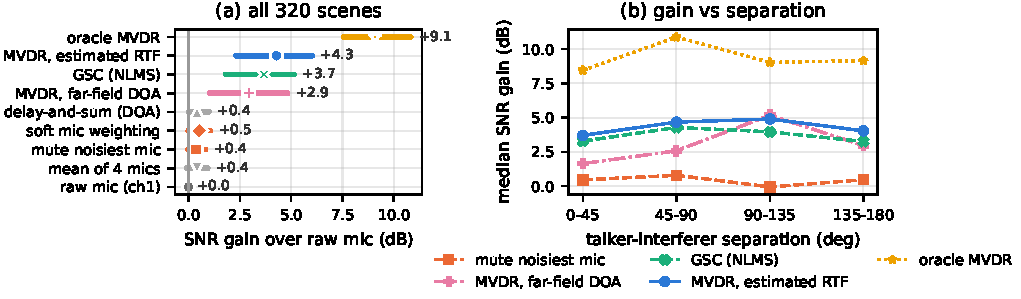
\includegraphics[width=\textwidth]{figures/spatial.pdf}
\caption{Exact SNR gain over the raw microphone (output minus input SNR on
ch1, the same weights applied to the true speech and noise components).
(a) Median and interquartile range over all \NScenes{} scenes. (b) Median
gain against the angle between talker and interferer as seen by the array,
each measured from its own clean take.}
\label{fig:spatial}
\end{figure*}

Figure~\ref{fig:spatial}a ranks the front ends by exact SNR gain.

\paragraph{Muting cannot work.} Switching off the noisiest microphone gains
\Gainmute\,dB and its per-band version \Gainmutesoft\,dB, no more than
simply averaging the four (\Gainmean\,dB). A far-field source reaches four
omnidirectional microphones within 6.4\,cm at the same level, so there is
no ``noisier'' microphone to drop. Delay-and-sum also gives
\Gainds\,dB: at speech frequencies the aperture is a fraction of a
wavelength, so phase alignment alone builds almost no directivity.

\paragraph{MVDR works.} The front ends that whiten the noise do:
\begin{itemize}
\item MVDR with an RTF from covariance whitening: \Gainmvdrrtf\,dB;
\item the adaptive GSC: \Gaingsc\,dB;
\item MVDR steered by the estimated direction: \Gainmvdrdoa\,dB.
\end{itemize}
The oracle MVDR, with the true noise covariance and speech RTF, reaches
\Gainoracle\,dB. That leaves about 5\,dB between what the silence model
supports and what the array could do. The gain holds across separations
(Fig.~\ref{fig:spatial}b), and is lowest when talker and interferer are
within 45$^\circ$ of each other.

\paragraph{Why the DOA-steered MVDR lags.} Its far-field steering depends
on a direction estimate (Fig.~\ref{fig:doa}). With an interferer at
0\,dB, the direction from the mixture minus the silence model is off by a
median \DoaErrSnrZero$^\circ$. At 10\,dB the error falls to
\DoaErrSnrOneZero$^\circ$. Steering by the RTF avoids the question: it
learns the talker's real transfer function, reverberation and near-field
included.

\begin{figure}[t]
\centering
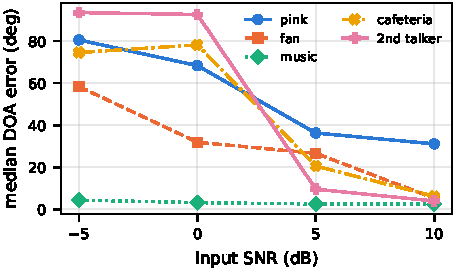
\includegraphics[width=\columnwidth]{figures/doa.pdf}
\caption{Talker direction estimated from the mixture (SRP-PHAT on mixture
minus silence model) against the direction from the clean take.}
\label{fig:doa}
\end{figure}

\subsection{Recognition: the attenuation limit}

\begin{figure*}[t]
\centering
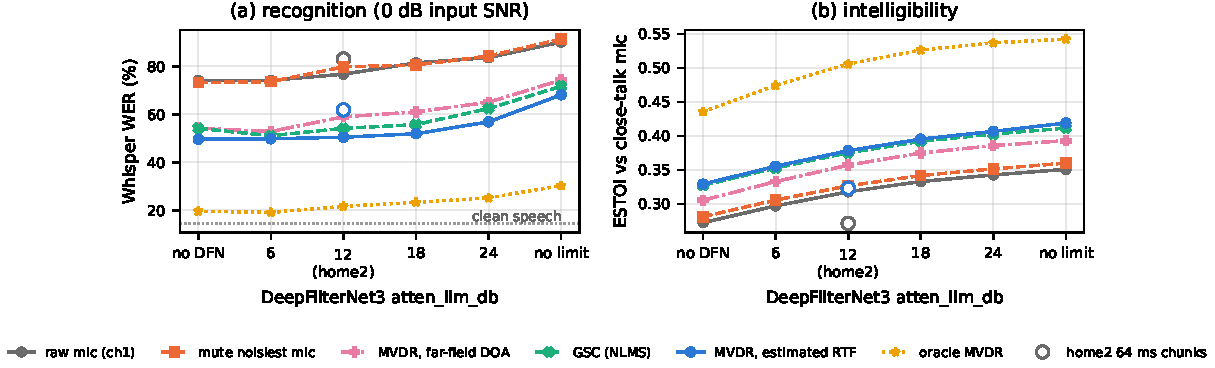
\includegraphics[width=\textwidth]{figures/atten.pdf}
\caption{All 0\,dB scenes (\NDfnScenes), each front end followed by
DeepFilterNet3 at every attenuation limit. (a) Whisper WER against the read
prompt; dotted: the same Whisper on the clean speech-only take. (b) ESTOI
against the close-talk microphone. Hollow markers: the robot's mode, with
independent 64\,ms chunks, at 12\,dB.}
\label{fig:atten}
\end{figure*}

Figure~\ref{fig:atten} shows the central result.

\paragraph{The front end dominates.} Without DeepFilterNet3, Whisper's WER
is \Werrefattoff\,\% on the raw microphone, \Wermuteattoff\,\% with the
mute, \Wergscattoff\,\% with the GSC and \Wermvdrrtfattoff\,\% with the RTF
MVDR. The paired difference against the raw microphone is \DiffRtfVsRef{}
points ($p=$\,\PRtfVsRef, Wilcoxon over scenes). With the oracle the WER is
\Weroracleattoff\,\%, close to the clean floor of \WerClean\,\%.

\paragraph{DeepFilterNet3 does not help the recognizer.} Its effect is the
same on every front end:
\begin{itemize}
\item At 6 and 12\,dB the WER barely moves: \DiffRefDfnTwelve{} and
  \DiffRtfDfnTwelve{} points at 12\,dB, $p=$\,\PRefDfnTwelve{} and
  \PRtfDfnTwelve.
\item From 18\,dB on, the WER rises: without a limit, by \DiffRefDfnInf{}
  and \DiffRtfDfnInf{} points.
\item Meanwhile ESTOI rises monotonically with the limit
  (Fig.~\ref{fig:atten}b).
\end{itemize}
This is the perceptual-versus-recognition split known from enhancement
artifacts~\cite{iwamoto2022artifacts}. For Whisper, the best limit is
``off'' to 12\,dB, and the robot's 12\,dB is at the safe edge.

\paragraph{The robot's chunked mode costs accuracy.} Enhancing each 64\,ms
chunk independently, peak-normalized, adds \DiffRtfHomeTwo{} points after
MVDR ($p=$\,\PRtfHomeTwo) and \DiffRefHomeTwo{} on the raw microphone
($p=$\,\PRefHomeTwo), relative to one continuous pass at the same limit.
The recurrent state of DeepFilterNet3 never warms up, and each chunk is
rescaled on its own.

\begin{figure}[t]
\centering
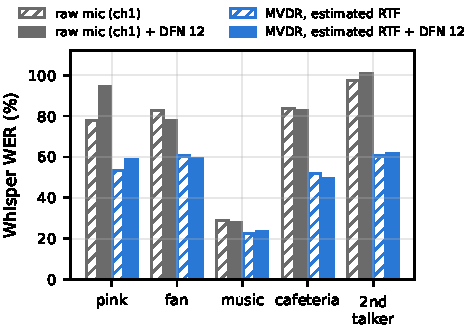
\includegraphics[width=\columnwidth]{figures/noise.pdf}
\caption{WER by interferer at 0\,dB SNR, raw microphone against RTF MVDR,
each without (hatched) and with DeepFilterNet3 at 12\,dB (solid).}
\label{fig:noise}
\end{figure}

\paragraph{By interferer} (Fig.~\ref{fig:noise}):
\begin{itemize}
\item The spatial front end helps most against the second talker
  (\Werrefattofftalker\,\% $\to$ \Wermvdrrtfattofftalker\,\%) and the
  cafeteria (\Werrefattoffcafeteria\,\% $\to$
  \Wermvdrrtfattoffcafeteria\,\%), the two interferers that are speech.
\item DeepFilterNet3 does not help even for stationary pink noise: on the
  raw microphone it raises the WER from \Werrefattoffpink\,\% to
  \WerrefattOneTwopink\,\%.
\item Music is the easiest interferer at equal SNR.
\end{itemize}

\subsection{Live takes}

\begin{figure*}[t]
\centering
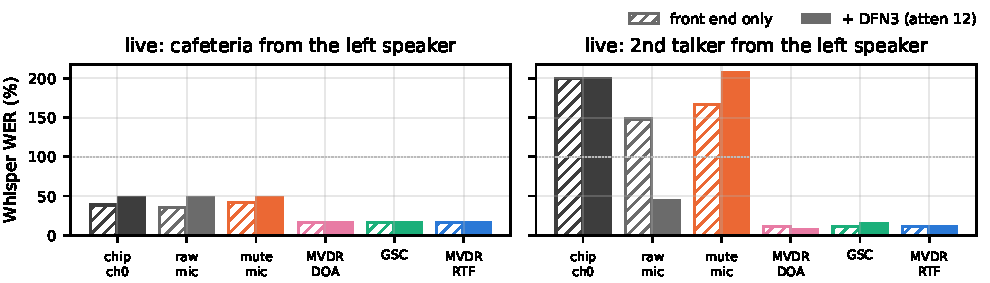
\includegraphics[width=\textwidth]{figures/live.pdf}
\caption{Live takes: the talker reads while an interferer plays from the
left speaker. Hatched: front end only. Solid: followed by DeepFilterNet3
at 12\,dB. ``chip ch0'' is the array's own processed channel, the robot's
current input. WER above 100\,\% means Whisper transcribed the interfering
voice.}
\label{fig:live}
\end{figure*}

\paragraph{Superposition check.} The talker live take replayed the same
interferer samples as its noise-only take. Before the talker speaks, the
live recording matches the scaled noise-only take with a residual of
\SuperResidual\,dB. Most of the residual sits below 300\,Hz, in room noise
that differs between takes. The rest comes from the talker's body and the
changed loudspeaker volume. Subtracting the matched interferer gives the
live speech component, and on it the RTF MVDR gains
\LiveGainmvdrrtf\,dB (DOA-steered: \LiveGainmvdrdoa\,dB; mute:
\LiveGainmute\,dB). These are somewhat below the mixed scenes, as the
residual suggests.

\paragraph{Live recognition} (Fig.~\ref{fig:live}). With an English
talker playing:
\begin{itemize}
\item On the chip's processed channel, with or without DeepFilterNet3,
  Whisper produces a Spanish rendering of the \emph{interfering} voice:
  WER \LivetalkerchZerochipDfn\,\%. The chip's own beam follows the louder
  voice.
\item The raw microphone with DeepFilterNet3 reaches
  \LivetalkerrefDfn\,\%.
\item Every phase-aware front end gets 7--15\,\%. The RTF MVDR followed by
  DeepFilterNet3 gets \LivetalkermvdrrtfDfn\,\%.
\end{itemize}
In the cafeteria take the beamformers reach \LivecafeteriamvdrrtfDfn\,\%,
against \LivecafeteriachZerochipDfn\,\% for the chip channel.

\section{Discussion}
\label{sec:discussion}

\paragraph{Hypotheses.}
\begin{itemize}
\item \textbf{H1, holds.} Muting or weighting microphones gains under
  1\,dB (\Gainmute{} and \Gainmutesoft\,dB, WER \DiffMuteVsRef{} points,
  $p=$\,\PMuteVsRef). Phase-aware front ends gain 3--4\,dB.
  \begin{itemize}
  \item We predicted \emph{at least 5\,dB} for MVDR. Only the oracle
    reaches that, so the bottleneck is the noise model from 1.5\,s of
    silence, not the array.
  \end{itemize}
\item \textbf{H2, half right.} The spatial front end matters most for
  speech-like interferers, as predicted. But DeepFilterNet3 alone does not
  ``handle'' stationary noise for the recognizer either: it improves ESTOI
  and leaves the WER flat or worse.
\item \textbf{H3, holds, but the optimum does not move.} WER is minimal
  from ``off'' to 12\,dB and grows beyond, both with and without a
  beamformer in front.
\item \textbf{H4, holds.} The robot's independent 64\,ms chunks cost 6--11
  points.
\end{itemize}

\paragraph{Falsification test.} We set this test in advance:
MVDR$\to$DeepFilterNet3 against DeepFilterNet3 alone at noise angles
$\geq$\,90$^\circ$. On those 44 scenes the difference is $-26.3$ WER
points, 38\,\% relative, far beyond the 10\,\% threshold. The difference is
the same below 90$^\circ$, and over all 0\,dB scenes it is
\DiffRtfDfnVsRefDfn{} points ($p=$\,\PRtfDfnVsRefDfn). The 4-microphone front end is worth adding.

\paragraph{Recommendations for the robot.}
\begin{enumerate}
\item Read the raw channels, not ch0.
\item Run an RTF-steered MVDR whose noise covariance is updated in the
  silence before each utterance. The voice activity detector already
  provides that silence.
\item Run DeepFilterNet3 continuously, or not at all, at 12\,dB or below.
  Never run it without a limit in front of the recognizer.
\end{enumerate}
The setting \texttt{atten\_lim\_db}\,=\,0 deserves a warning, because the
library reads it as ``no limit''.

\paragraph{Limitations.}
\begin{itemize}
\item One talker, one room and one session. The talker's angle marks were
  approximate, so separations come from the clean takes.
\item Scenes are mixed. The live check shows they are optimistic by 1--2\,dB
  of SNR gain, but the two live takes agree with them in direction and size.
\item Whisper \texttt{small} with greedy decoding; a larger model is more
  noise-robust and may shrink every gap.
\item The 0\,dB scenes are hard on purpose: the absolute WERs are high, the
  differences are what matters.
\item The cafeteria live take could not be checked for superposition: a
  bug in the noise generator replayed a different excerpt.
\end{itemize}

\paragraph{Project~15.} The same session gives project~15 its missing
hardware numbers:
\begin{itemize}
\item \textbf{Orientation.} The array is mirrored and rotated by
  \PFifteenOffset$^\circ$ relative to the talker's marks.
\item \textbf{Direction.} The leave-one-out median error is
  \PFifteenLooErr$^\circ$, bounded by the marks' accuracy.
\item \textbf{Distance fails.} No distance cue correlates with distance
  (|Spearman|\,$\leq$\,\PFifteenSpearmanMax). The best model's error is
  \PFifteenMaeBest\,m, against \PFifteenMaeMean\,m for predicting the mean.
\end{itemize}

\section{Conclusion}
\label{sec:conclusion}

On a 4-microphone ReSpeaker, directional noise cancellation has to come
from combining the microphones with phase. Switching one off does nothing.
An MVDR beamformer steered by a transfer function learned in the silence
before the talker speaks cuts Whisper's word error rate by a third at 0\,dB
SNR. Against a second voice, it is the difference between transcribing the
talker and transcribing the television.

DeepFilterNet3 does not add to recognition at any attenuation limit.
Above 12\,dB, and in the robot's chunked mode, it subtracts, even as
intelligibility metrics improve. The limit should be set for the
recognizer, not by ear, and the array should be pointed before the
denoiser is turned up.


\FloatBarrier
\bibliographystyle{plain}
\bibliography{references}
\end{document}
